\documentclass[8pt]{beamer}
\usetheme{default} % Very simple theme
\usecolortheme{dove} % Minimalist grayscale colors
\setbeamertemplate{navigation symbols}{} % Remove navigation bar

% Define brand-like colors
\definecolor{myblue}{RGB}{0, 102, 204}    % Blue for standard blocks
\definecolor{mygreen}{RGB}{0, 153, 0}     % Green for example blocks
\definecolor{myred}{RGB}{204, 0, 0}       % Red for alert blocks

% Accent color for titles, bullets, etc.
\setbeamercolor{structure}{fg=myblue}

% Block colors
\setbeamercolor{block title}{bg=myblue, fg=white}
\setbeamercolor{block body}{bg=blue!5, fg=black}

\setbeamercolor{exampleblock title}{bg=mygreen, fg=white}
\setbeamercolor{exampleblock body}{bg=green!5, fg=black}

\setbeamercolor{alertblock title}{bg=myred, fg=white}
\setbeamercolor{alertblock body}{bg=red!5, fg=black}

% Optional: color for \example text
\setbeamercolor{example text}{fg=mygreen}
\usepackage{graphicx} % Package for images
\usepackage{amsmath} % Package for images
\graphicspath{{figs/}} % Path to your figures directory
\usepackage{array}  % For better column spacing
\usepackage{caption} % Required for \captionof

% Title Information
\title{Stochastic methods in water resources}
\subtitle{Lecture 3: xxxx}
\author{Luis Alejandro Morales, Ph.D.}
\institute{Universidad Nacional de Colombia} %// Department of Civil and Agriculture Engineering}
\date{\today}

\begin{document}

% Title Slide
\begin{frame}
    \titlepage
\end{frame}

%-------
% From Kotte
\section{Generalities}
\begin{frame}{Generalities}
    \begin{itemize}
        \item Natural and artificial hydrosystems exhibit large variability in space and time, so deterministic laws can not explain them completely.
        \item A hydrological variables is thus considered as a \alert{random variable} as it is not explain totally based on other variables. 
        \item By incorporating \emph{probability theory} is possible to deal with a random variable's uncertainty. 
        \item Outcome of mathematical models aimed to represent real world processes (e.g. the Richard's equation to model groundwater flow) are uncertain as  model's independent variables come from experiments (e.g. rain gauge) and model's parameters change within a range. Also,  model's structure might not represent correctly the physical phenomena so it exhibits uncertainty. 
        \item It would be desirable to build precise models to predict the occurrence of an event, but this is not possible. So, probability models are build to determine the likelihood of the occurrence of an event. 
        \item However, the uncertainty estimates of a hydrological random variables is limited by:
            \begin{itemize}
                \item Inherent nature's variability
                \item Insufficient knowledge of governed hydrological laws
                \item Quantity and quality of data.
            \end{itemize}
    \end{itemize}
\end{frame}

%-------
% From Kotte
\section{Random events}
\subsection{Sample space and events}
\begin{frame}{Sample space and events}
    \begin{block}{Random event ($A$)}
        A \emph{random event} is an outcome of an experiment where observations are taken under fair conditions and no bias are expected toward a particular result. It can be a collection of points in $\Omega$.
    \end{block}
    \begin{block}{Sample space ($\Omega$)}
        The \emph{sample space}, also known as the \emph{universe} or the \emph{population}, is a set with the collection of all the observations (or all the possible values) of a variable within an experiment. Each point in the sample space is a \emph{sample point} and one or more points can constitute an event. An event is thus a subset of $\Omega$.  
    \end{block}
    % Ex 2.1. Kotte
    \begin{exampleblock}{Reservoir storage}
    In a reservoir that store an amount of water of $S$, water level varies from 0 to $c$. Water level storage is divided into: \emph{depth storage}, \emph{supply storage} and \emph{flood-control storage} (see the figure).
    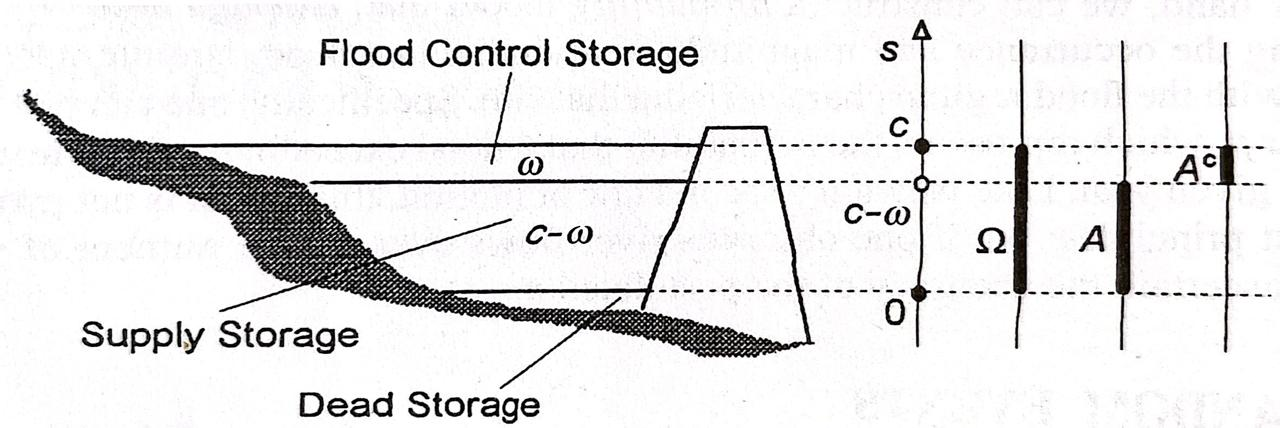
\includegraphics[width=0.7\textwidth]{fi211.jpeg}
    Accordingly, the sample space, $\Omega$, is the storage at a given time defined as $\Omega \equiv {S: 0 \leq S < c}$. Note that, $\Omega$ is continuous on $[0,x)$, there is an infinite number of points. However $\Omega$, can be divided into a discrete number of states depending of the engineer's judment. 
    \end{exampleblock}
        
\end{frame}

\begin{frame}{Sample space and events}
    \begin{exampleblock}{Reservoir storage}

    \begin{minipage}{0.59\textwidth}
        Consider four states ($\omega$) of a reservoir storage $S$, so $\omega_i \equiv {S: (i-1)c/4 \leq S < ic/4}$, $i = 1, \cdots, 4$.
        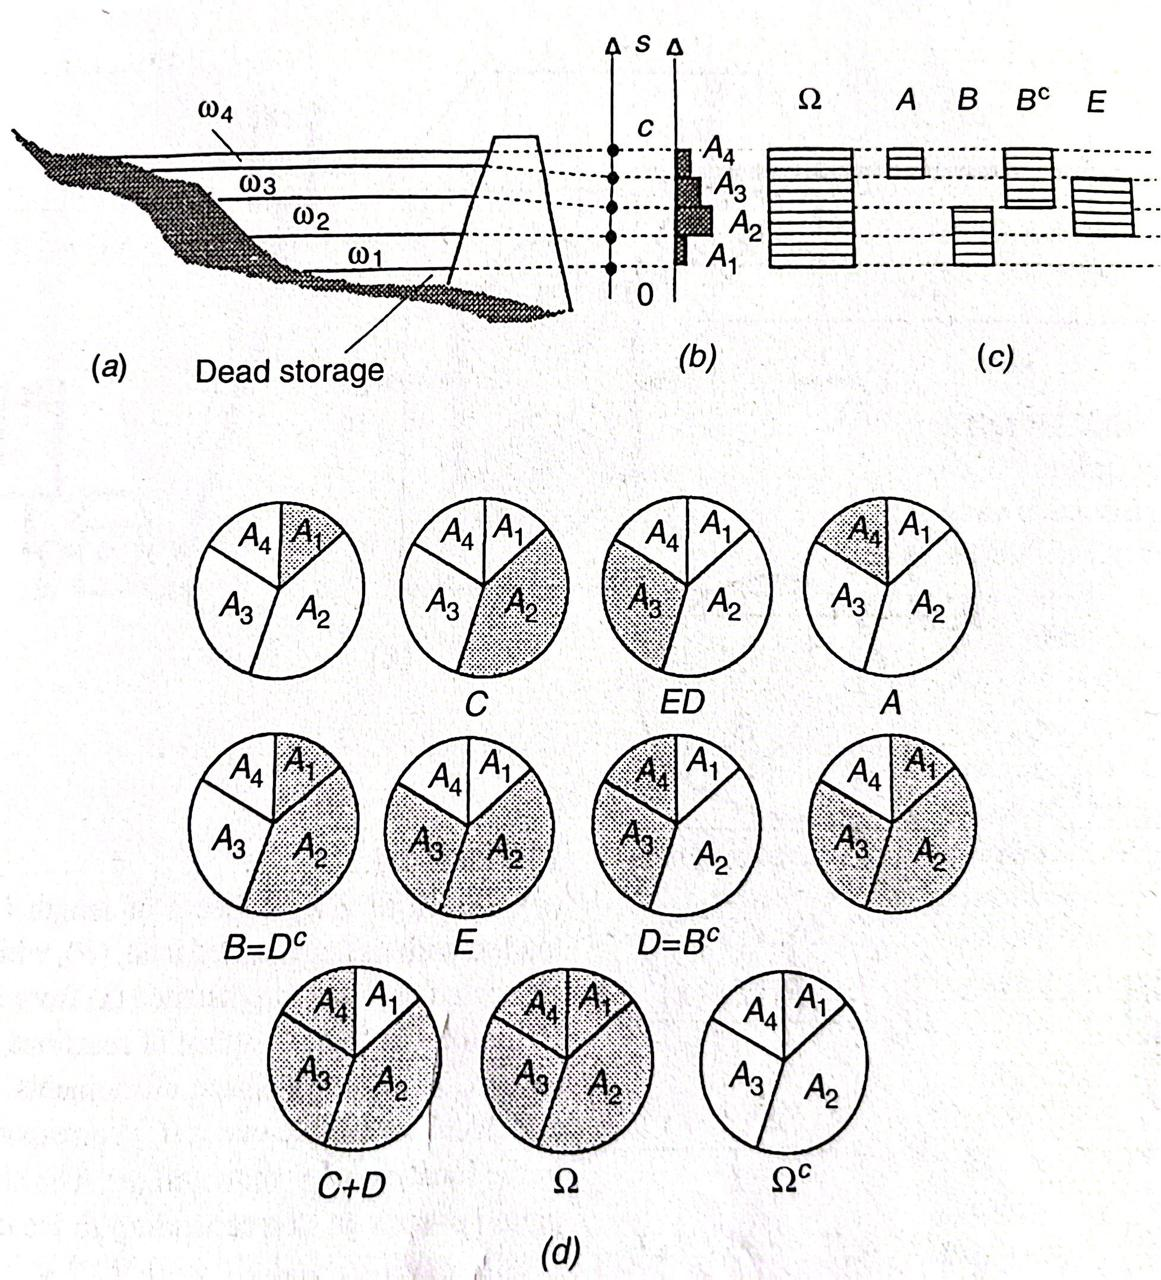
\includegraphics[width=\textwidth]{fi212.jpeg}
    \end{minipage}
    \hfill
    \begin{minipage}{0.39\textwidth}
        In the figure, a) represents the four storage states; b) is the frequency of the states; c) is the events of interest that combine states, where rectangle width is proportional to the state frequency, and d) shows pie charts of all possible events (shaded area) based on the four states. For instance, the simple event $A = \omega_4 \equiv A_4$ implies that $3c/4 \leq S < c$. The event $A = \omega_1 + \omega_2 \equiv B \equiv {S: 0 \leq S < c/2}$ is a compound event because it comprise of two single events, $A_1 \equiv {S: 0 \leq S < c/4}$ y $A_2 \equiv {S: c/4 \leq S < 2c/4}$.
    \end{minipage}
    \end{exampleblock}
    In general, $A$ is subset of $\Omega$ ($A \subset \Omega$) and $A^c$ is the complement of $A$ that consist of all outcomes of $\Omega$ that are not in $A$.
 
\end{frame}

\subsection{Null event, intersection and union}
\begin{frame}{Null event, intersection and union}
    Events in $\Omega$ can be related in different ways. Here is some definitions:
    \begin{block}{Mutually exclusive events}
        If $A_1$ and $A_2$ are events in $\Omega$, they are \emph{mutually exclusive} or \emph{disjoint} if the occurrence of one event excludes the occurrence of the other. This means, for instance, that none of the points in $A_1$ are in $A_2$ or vice versa. In this case, the \emph{null} event is constituted by $A_1$ and $A_2$ and denote as $A_1 A_2 = A_1 \cap A_2 = \varnothing$. In the reservoir storage example, $A$ and $B$ are mutually exclusive and, in general, all the $\omega_i$ events.  
    \end{block}

    \begin{block}{Intersection}
        An \emph{intersection} is constituted by all the common sample points in $A$ events, it means, points that are in all the $A_i$ events. These events are also not mutually exclusive. If two events $A_1$ and $A_2$ are not mutually exclusive, their intersection is denoted by $A_1 \cap A_2$ so that $A_1 \cap A_2 \neq \varnothing$. In the reservoir storage example, $A \cap B^c$ is the event ${S: 3c/4 \leq S < c}$ which correspond to $\omega_4$. 
    \end{block}

    \begin{block}{Union}
        The union of $A$ events constitutes their joint occurrence and it comprises an event that contain all the sample points in $A$s. If we have two events $A_1$ and $A_2$, their union is denoted as $A_1 \cup A_2$ ($A_1 + A_2$). For instance, in the reservoir storage example, the states or events $A_1 = \omega_1$ and $A_2 = \omega_2$ constitute the $B$ event, so $B = A_1 \cup A_2$.
    \end{block}
    Note that event intersections and unions can create new events within $\Omega$. 
\end{frame}


\subsection{Venn diagram and event space}
\begin{frame}{Venn diagram and event space}
    To undestand the Venn diagram is important consider the following:
    \begin{itemize}
        \item A \emph{set} is a collection of points in a sample space $\Omega$.
        \item A Venn diagram provides a visual representation of set operations such as: complement, union, intersection and combinations of them. 
        \item Sample points, sample spaces and events are sets.
    \end{itemize}
    \begin{block}{Event space}
         The \emph{event space} ($\wp$) is constituted by all possible event combinations. This means, all possible outcomes of the experiment included in $\Omega$. For instance, the pie charts in the reservoir storage example. $\wp$ has the following properties:
         \begin{enumerate}
             \item $\Omega \in \wp$ 
             \item If $A \in \wp$, then $A^c \in \wp$ 
             \item If $A_1 \in \wp$ and $A_2 \in \wp$, then $A_1 + A_2 \in \wp$
             \item If $\varnothing \in \wp$, then $A^c \in \wp$
             \item If $A_1 \in \wp$ and $A_2 \in \wp$, then $A_1 A_2 \in \wp$
         \end{enumerate}
         For instance, the event space of the reservoir storage example is:
         $$
         \begin{aligned}
             \wp &= \{ A_1, A_2, A_3, A_4, A_1 + A_2, A_2 + A_3, A_3 + A_4, A_1 + A_2 + A_3, \\
                 & A_2 + A_3 + A_4, A_1 + A_2 + A_3 + A_4, \varnothing \}
         \end{aligned}
         $$
    \end{block}
\end{frame}

\begin{frame}{Venn diagram and event space}

    \begin{minipage}{0.59\textwidth}
        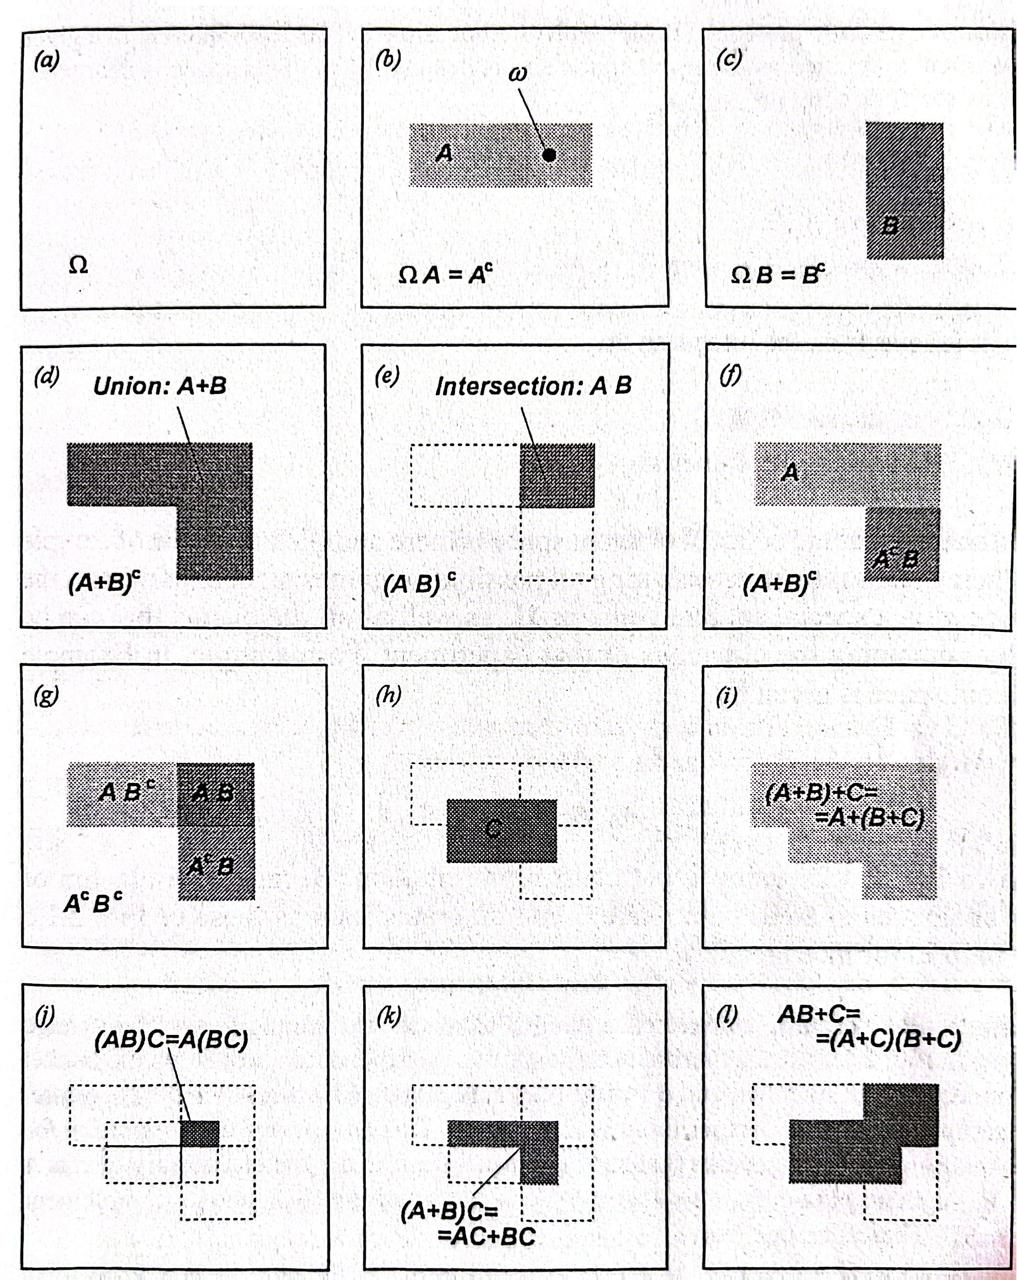
\includegraphics[width=0.9\textwidth]{fi216.jpeg}
    \end{minipage}
    \hfill
    \begin{minipage}{0.39\textwidth}
        \begin{itemize}
            \small
            \item a) is the sample space $\Omega$ constituted by all possible experiment outcomes.
            \item c) and b) show the simple events (shaded rectangles) $A$ and $B$. Note that $\omega$ represent an outcome of the event $A$.
            \item d) and e) show the union ($A+B$) and the intersection ($A \cap B$ = AB), respectively. 
            \item f) and g) show the $A^c B$ and the $A B^c$ events.
            \item h) shows event $C$ that intersects $A$ and $B$.
            \item i) and j) show the following compound events (\emph{associative})
                \vspace{-5pt}
                $$
                \begin{aligned}
                &(A + B) + C = A + (B + C) \\
                &(A \cup B) \cup C = A \cup (B \cup C)
                \end{aligned}
                $$
                $$
                \begin{aligned}
                &(AB)C = A(BC) \\
                &(A \cap B) \cap C = A \cap (B \cap C)
                \end{aligned}
                $$
            \item k) and l) show the following compound events (\emph{distributive})
                \vspace{-5pt}
                $$
                \begin{aligned}
                &(A + B)C = AC + BC \\
                &(A \cup B) \cap C = (A \cap C) \cup (B \cap C)
                \end{aligned}
                $$
                $$
                \begin{aligned}
                    &AB + C = (A + C)(B + C) \\
                    &(A \cap B) \cup C = (A \cup C) \cap (B \cup C)
                \end{aligned}
                $$
        \end{itemize}
    \end{minipage}

\end{frame}

\begin{frame}{Some examples}

    \begin{exampleblock}{Reservoir storage}
        The continuous sample space of a reservoir storage is denoted by $\Omega \equiv \{ S: 0 \leq S < c \}$, where maximum storage is $c$. Accordingly, the event space can be defined as $\wp \equiv \{ S: x \leq S < y \}$, where $0 \leq x \leq y < c$ for any pair of $x$ and $y$ in $[0,c)$. Lets consider the following events: $A \equiv \{ S: 0 \leq S < c/3 \}$, $B \equiv \{ S: c/4 \leq S < c/2 \}$ and $C \equiv \{ S: c/5 \leq S < 3c/5 \}$. The following events are defined using event's algebra:
        \begin{itemize}
            \item $AB \equiv A \cap B \equiv \{ S: c/4 \leq S < c/3 \}$ 
            \item $A + B \equiv A \cup B \equiv \{ S: 0 \leq S < c/2 \}$ 
            \item $(A + B) C = AC + BC \equiv \{ S: c/5 \leq S < c/2 \}$ 
            \item $AB + C = (A + C) (B + C) \equiv C \equiv \{ S: c/5 \leq S < c/2 \}$ 
        \end{itemize}

    \end{exampleblock}
    In engineering, problems sometimes involve data from join observations, that in many cases are recorded at the same time and location. For instance: \emph{Dissolved oxygen and biochemical oxygen demand in stream waters to assess river pollution}, \emph{Intensity and duration of storm rainfalls at a rain gauge} and \emph{Wind speed and direction at a weather station}. All these cases involve two variables whose 2D sample space can be discrete, continuous or both. 

    Commonly, there is interest in the possible outcomes of an experiment given that event $A$ has occurred. This means that as $A$ has occurred, the sample space is restricted or conditioned to the set representing $A$. For instance, if an engineer is interested in sea waves exceeding 2m in height ($h$) and wave direction ranging from 25$^o$ to 120$^o$, the original sample space $\Omega \equiv \{ (h, \theta) : h > 0 \text{ and } 0^o \leq \theta \leq 360 \}$    is thus reduced. This concept of \emph{conditional sample space} will be relevant to the study of \emph{conditional probabilities}.  
\end{frame}

\begin{frame}{Some examples}
    \begin{minipage}{0.59\textwidth}
    \begin{exampleblock}{Number of rainy days and total rainfall}
        Let's say that one is interested in the number of rainy days  and the total amount of rainfall in a period between the first and the 10th of September (10 days) nearby Bogota, in an agricultural region subjected to irrigation. If there is rain gauge at the location of interest, the sample space is defined as $\Omega \equiv \{ (i, x): i = 0, 1, 2, \cdots, 10; \text{ and } 0 \leq x\}$, where $i$ is the number of rainy days and $x$ is the total rainfal during $i$ in millimeters. For instance, farmers know that if the $i>3$ days and $x > 20$ mm  no irrigation is needed. These random events can be denoted as $A \equiv \{ (i, x) : i > 3 \text{ and } x > 20 \}$. Note that event $A^c \equiv \{ (i, x) : i < 4 \text{ and } x \leq 20 \}$ is the event where irrigation is required. Supposed that there are two mutually exclusive events that describe two different circumstances: $B \equiv \{ (i, x) : 3 \leq i < 5 \text{ and } x \geq 10 \}$ and $C \equiv \{ (i, x) : 1 \leq i < 3 \text{ and } 2 \leq x < 10 \}$. In this case $AB = \varnothing$. According to algebra of events, the following new events can be established also part of the event space $\wp$
        \begin{itemize}
            \item $A + B \equiv \{ (i, x) : i > 2 \text{ and } x \geq 10 \}$
            \item $B + C \equiv \{ (i, x) : 1 \leq i < 5 \text{ and } x \geq 2 \}$
            \item $AB \equiv \{ (i, x) : i = 4 \text{ and } x > 20 \}$
        \end{itemize}
        
    \end{exampleblock}
\end{minipage}
\hfill
    \begin{minipage}{0.39\textwidth}
        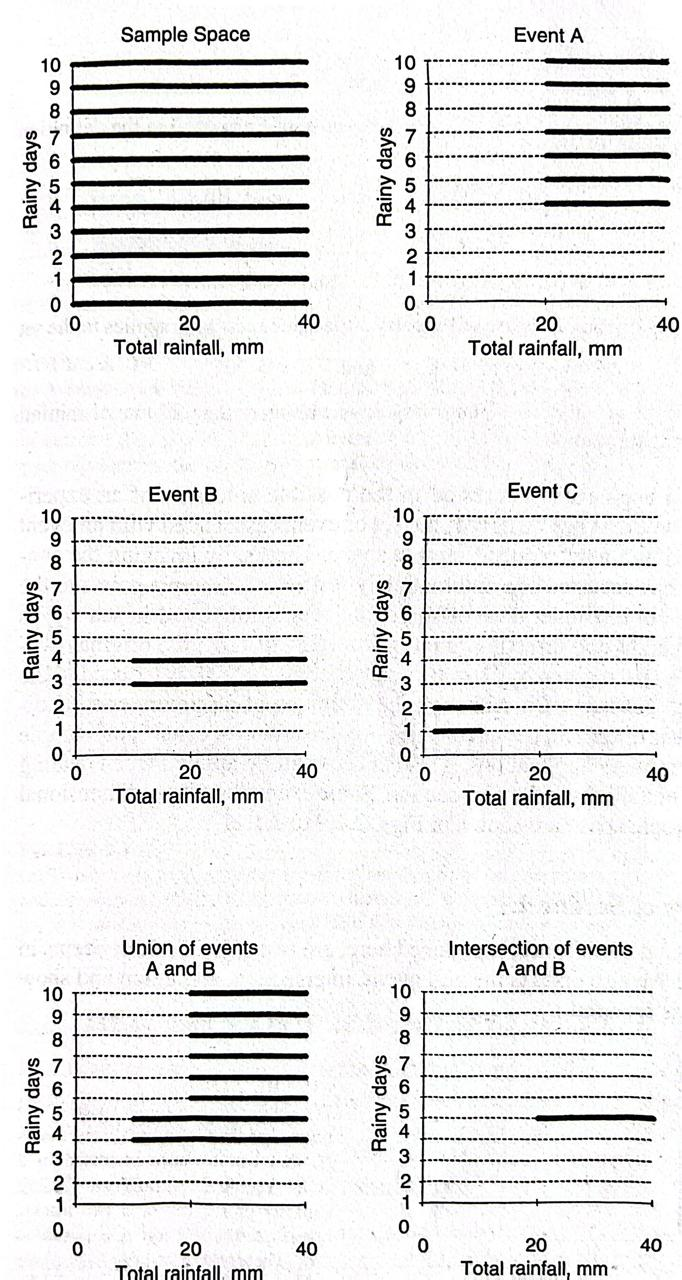
\includegraphics[width=0.9\textwidth]{fi218.jpeg}
    \end{minipage}
\end{frame}


\section{Probability theory}
\subsection{Interpretation of probability}
\begin{frame}{Interpretation of probability}
    \begin{block}{Probability}
        \emph{Probability} is a math branch that deal with random events. For instance, the random experiment of tossing a coin $n$ times results in $n$ \emph{mutually exclusive} and \emph{equally likely} outcomes, and for $n_A$, that correspond to a certain attribute $A$ (e.g. coin tail or coin head), the probability of obtaining $A$ is $n_A / n$. If $A$ represents coin tail and $B$ represents coin head, the probability of $A$ and $B$ using a fair coin is 0.5 for both. This probability is called \emph{prior probability} as it is obtained from deductive reasoning and not requires verification. In the case of a no fair coin, it is not possible to know the prior probability as the $A$ and $B$ are not equally likely. So asking about the probability of obtaining tail or head is like asking, what is the probability that tomorrow will be a rainy day? or, what is the probability that a hurricane hits Florida next year?. To answer this questions the \emph{posterior probability} or \emph{frequency} needs to be estimated based on previous observations under uniform/stable conditions. For discrete variables like the number of rainy days in a year, the \emph{relative frequency}, $p$, is  estimated for each number of rainy days from the historical data. In the case of continuous variables, $p$ is estimated within a range, let's say, the probability that daily rainfall is greater than 20 mm and lesser than 50 mm. There are cases in which the situation for analysis do not fit into the framework of repeated outcomes within the experiment. For instance, what is the probability that the Chingaza system meets the water demand for the next 25 years?  This kind of problems are part of what is known \emph{subjective probability} that contrasts with objective methods based on theory or observation. Subjective probabilities are assigned based on experience and personal judgement and play an important role in the \emph{Bayesian approach}. 
    \end{block}
\end{frame}

\begin{frame}{Probability axioms}
    \begin{block}{Probability axioms}
        Probability theory is founded on the \emph{probability axioms} and are applied to prior, posterior or subjective probabilities. To define the axioms is necessary to define a \emph{function}, $f$. A function is a mathematical rule that associate/map one value or point from the \emph{domain} with one and only one value or point in the \emph{counterdomain}.  For instance in the reservoir example, the water level $h$ can take values from $h_min \leq h < h_sup$ (domain). This values can be mapped by the stage-volume function $s = f(h)$ to estimate the storage $s$ whose counterdomain is $0 \leq s < c$. Recalling the concepts of \emph{sample space} and \emph{event space}, in probability theory, a \emph{probability function}, $P_r$, is a function whose domain is $\wp$ and the counterdomain is $0 \leq Pr \leq 1$. This means that the probability of, let's say an event $A$ ($P_r [A]$) in $\wp$ is a mapped value within $[0,1]$. In terms of $\Omega$, $Pr[A]$ is the sum of all the probabilities of the sample points in $A$. For continuous variables where $\Omega$ is constituted by infinite number or points, probabilities are assigned to areas or lenghts. The probability axioms are:
        \begin{enumerate}
            \item $Pr[A] \geq 0, \text{ for every } A \in \wp$
            \item $Pr[\Omega] = 1$
            \item If $A_1 \in \wp$, $A_2 \in \wp$, and $A_1 A_2 = \varnothing$, then $Pr [A_1 + A_2] = Pr[A_1] + Pr[A_2]$ 
        \end{enumerate}
        where $A$, $A_1$ and $A_2$ are events that belong to the sample space.  
    \end{block}
\end{frame}

\begin{frame}{Probability axioms}
    \begin{exampleblock}{Reservoir storage}
        In the previous reservoir storage example, the reservoir storage $S$ was discretized into four states: $\omega_1$, $\omega_2$, $\omega_3$ and $\omega_4$, where the sample space is the set $\Omega \equiv \{A_1, A_2, A_3, A_4 \}$, so $A_i \equiv \omega_i \equiv \{ S: (i-1)c/4 \leq S \leq ic/4 \}$ for $i = 1, 2, 3, 4$. As observation of reservoir storage is made at the end of the operation year, 36 measures of $S$ has been recorded. The frequency analysis yields the following occurrence of $A_i$: $A_1 = 5$, $A_2 = 15$, $A_3 = 10$ and $A_4 = 6$. According with the \alert{axiom 1}:
        $$
        Pr[A_1] = \frac{5}{36} \quad Pr[A_2] = \frac{15}{36} \quad Pr[A_3] = \frac{10}{36} \quad Pr[A_4] = \frac{6}{36} 
        $$
        \alert{Axiom 2} is satisfied as:
        $$
        Pr[\Omega] = Pr[ A_1 + A_2 + A_3 + A_4 ] = \frac{5}{36} + \frac{15}{36} + \frac{10}{36} + \frac{6}{36} = 1
        $$
        If we consider two mutually exclusive events: $C = A_2 \equiv \{ S: c/4 \leq S < c/2 \}$ and $D = A_3 + A_4 \equiv \{ S: c/2 \leq S < c \}$, $C + D = A_2 + A_3 + A_4$, so:
        $$
        Pr[C + D] = Pr[ A_2 + A_3 + A_4 ] = \frac{15 + 10 + 6}{36} = \frac{15}{36} + \frac{16}{36} = Pr[C] + Pr[D]
        $$
        This satisfy \alert{axiom 3}. 
    \end{exampleblock}
\end{frame}

\begin{frame}{Addition rule}
    The axiom 3 can be extended to any sequence of mutually exclusive events $A_1, A_2, \cdots, A_k \, \in \wp$, so that, $A_i A_j = \varnothing$ for any $i \neq j$ where $i,j = 1, 2, \cdots, k$. Axiom 2 can be applied to an event $A$ and to its complement $A^c$. As $A$ and $A^c$ are mutually exclusive events, $Pr[A + A^c] = Pr[A] + Pr[A^c] $. If $A + A^c = \Omega$, $Pr[A + A^c] = Pr[\Omega] = 1$. From this, the \emph{probability of the complement of A} is $Pr[A^c] = 1 - Pr[A]$.
    \begin{exampleblock}{Flood occurrence}
        Suppose that one want to analyse the number of flood occurrences, $N$,  per year. Accordingly, the engineer is interested in evaluating the likelihood of the ocurrence of such a flood in any year. If $\Omega \equiv \{ N : N \geq 0 \}$ and $A \equiv \{ N : N > 0 \}$ (occurrence of at least one flood), therefore, $A^c \equiv \{ N : N = 0 \}$ (occurrence of no floods). According to annual records of floods in a river gauge station between 1936 and 1995, six floods occurred in: 1945, 1951 (twice), 1953, 1970 and 1992. So that, the probability of flood ocurrence is $Pr[A] = \frac{6}{65} = 0.092$ and the probability of no floods is $Pr[A^c ] = 1 - Pr[A] = 1 - \frac{6}{65} = 0.908$. $Pr[A] = 0.092$ indicates the likelihood of the occurrence of at least one flood and it is a measure of the risk affecting the river nearby area. 
    \end{exampleblock}
\end{frame}

\begin{frame}{Addition rule}
    Suppose that we have two events, $A$ and $B$, that are not necesarily mutually exclusive. Accordingly, $A + B = A + A^c B$, so $A$ and $C = A^c B$ are mutually exclusive. Using the axiom 3:
    $$
    Pr[A + B] = Pr[A + A^c B] = Pr[A] + Pr[A^c B] = Pr[A] + Pr[C]
    $$
    Similarly, $Pr[B]$ can be estimated as:
    $$
    Pr[B] = Pr[A^c B] + Pr[AB]
    $$
    Replacing in the equation above, the \emph{addition rule} establishes that:
    $$
    Pr[A + B] =  Pr[A] + Pr[B] - Pr[AB]
    $$

    If $A$ and $B$ are mutually exclusive events ( $AB = \varnothing$ ), $Pr[AB] = 0$, so:
    $$
    Pr[A + B]  = Pr[A] + Pr[B]
    $$
\end{frame}

\begin{frame}{Further properties of probability functions}

    \begin{block}{Probabilty of null event}
        The probability of the \emph{null} event is zero, this means
        $$
        Pr[\varnothing] = 0
        $$
    \end{block}
    \begin{block}{Probabilty of a contained event}
        If an event $A$ is contained in a event $B$, the probability of $A$ does not exceed the probability of $B$. This means:
        $$
        Pr[A] \leq Pr[B] \quad \text{ if } A \subset B
        $$
    \end{block}
    \begin{block}{Boole's inequality}
        If there is $n$ events $A_i$ where $i = 1, 2, \cdots, n$, the probability of the union of the $n$ events does not exceeed the sum of their probabilities, that is:
        $$
        Pr[A_1 + A_2 + \cdots + A_n] \leq Pr[A_1] + Pr[A_2] + \cdots + Pr[A_n]
        $$
    \end{block}
\end{frame}

\begin{frame}{Further properties of probability functions}
    \begin{exampleblock}{Dam failure}
        In a earthquake-prone area, the failure of dam can be produced by two events: Event $A$ means the occurrence of large flood exceeding the capacity of the dam's spillway, and event $B$ means a severe, destructive earthquake that cause the collapse of the dam. The analysis performed by the consultant yields that the $Pr[A] = a$ (flood exceeding) and $Pr[B] = b$ (earthquake occurrence). Accordingly, the probability of dam's failure is given by:
        $$
        Pr[A + B] = Pr[A] + Pr[B] - Pr[AB]
        $$
        However, the joint event $AB$ is quite improbable. According to the \emph{Boole's inequality}:
        $$
        Pr[A + B] \leq Pr[A] + Pr[B]
        $$
        This is equivalent to 
        $$
        Pr[A + B] \approx Pr[A] + Pr[B] = a + b
        $$
        According to the literature, the values of $a$ and $b$ are 0.02 and 0.01, respectively, so:
        $$
        Pr[A + B] \approx 0.02 + 0.01 = 0.03
        $$
        This indicate that the probability of the dam's collapse is around 3\% in a given year. 
    \end{exampleblock}
\end{frame}

\subsection{Conditional probability and multiplication rule}
\begin{frame}{Conditional probability and multiplication rule}
    
    In many practical application, it is required to inquiry the probability of an event given the occurrence of one or more events; this is known as the \emph{conditional probability}. For instance, given that a dam has not failed in the last 100 years, one is interested in the probability of no failure of the dam for another 100 years. For instance, given that high streamflow in a river have been observed in January, February and March, an engineer may be interested in the probability of that streamflow will exceed 2000 m$^3$/s in April. The questions in these examples can be solved only using the concept of \emph{conditional probability}. 
    \begin{block}{Conditional probability}
        Let $A$ and $B$ two events in the sample space $\Omega$ of an experiment. Given that the $Pr[B] > 0$, the \emph{conditional probability} of event $A$ given that $B$ has ocurred, is defined as:
        $$
        Pr[A | B] = \frac{Pr[AB]}{Pr[B]}
        $$
        where $Pr[B] = 0$ means that $Pr[A | B]$ is undefined. Note that $\Omega$ is reduced to $B$ and $Pr[B]$ is known and the \emph{marginal probability} of event $B$. According to the frequency approach to estimate probabilities, $Pr[A | B]$ can be calculated as:
        $$
        Pr[A | B] = \frac{Pr[AB]}{Pr[B]} = \frac{n_{AB} /n}{n_b /n} = \frac{n_{AB}}{n_b}
        $$
        where $n_{AB}$ and $n_B$ are the number of $AB$ and $B$ events, respectively, and $n$ is the total number of events. 
    \end{block}
\end{frame}

\begin{frame}{Conditional probability and multiplication rule}
    
    \begin{block}{Conditional probability}
        There are cases where $Pr[A | B]$ and $Pr[B]$ can be estimated directly, whereas the join probability $Pr[AB]$ is unknown. This can be estimated as:
$$
Pr[AB] = Pr[A | B] Pr[B] = Pr[B | A] Pr[A]
$$
From \alert{axiom 2}, $Pr[A | B] \leq 1$ and $Pr[B | A] \leq 1$, the following inequalities also hold:
$$
Pr[A | B] \leq \frac{Pr[A]}{Pr[B]} \quad Pr[B | A] \leq \frac{Pr[B]}{Pr[A]}
$$
        \end{block}

    \begin{block}{Multiplication rule}
        The concept of conditional probability can be extended to any number of events. For instance for events $A$, $B$ and $C$:
        $$
        Pr[ABC] = Pr[A | BC] Pr[BC] = Pr[A | BC] Pr[B | C] Pr[C]
        $$
        For $m$ events, the joint probability of the $m$ events is:
$$
Pr[A_1 A_2 A_3 \cdots A_m ] = Pr[A_1 | A_2 A_3 \cdots A_m ] Pr[A_2 | A_3 A_4 \cdots A_m] \cdots Pr[A_m]
$$
This is known as the \emph{multiplication rule} of probability theory. This rule is useful for experiments defined in terms of stages (e.g successive events). 
        \end{block}

\end{frame}

\begin{frame}{Conditional probability and multiplication rule}
    \begin{exampleblock}{Water distribution}
        Suppose that in a city whose surface area is approximately flat and rectangular with sides 10 km and 20 km and area of 200 km$^2$, there is aquaduct network where pipes are distributed according to the figures. The city area is uniformely covered by the network so that, pressure and flow rates are uniform trhoughout the network. Accordingly, the probability of water loss in any network segment is equal. 
        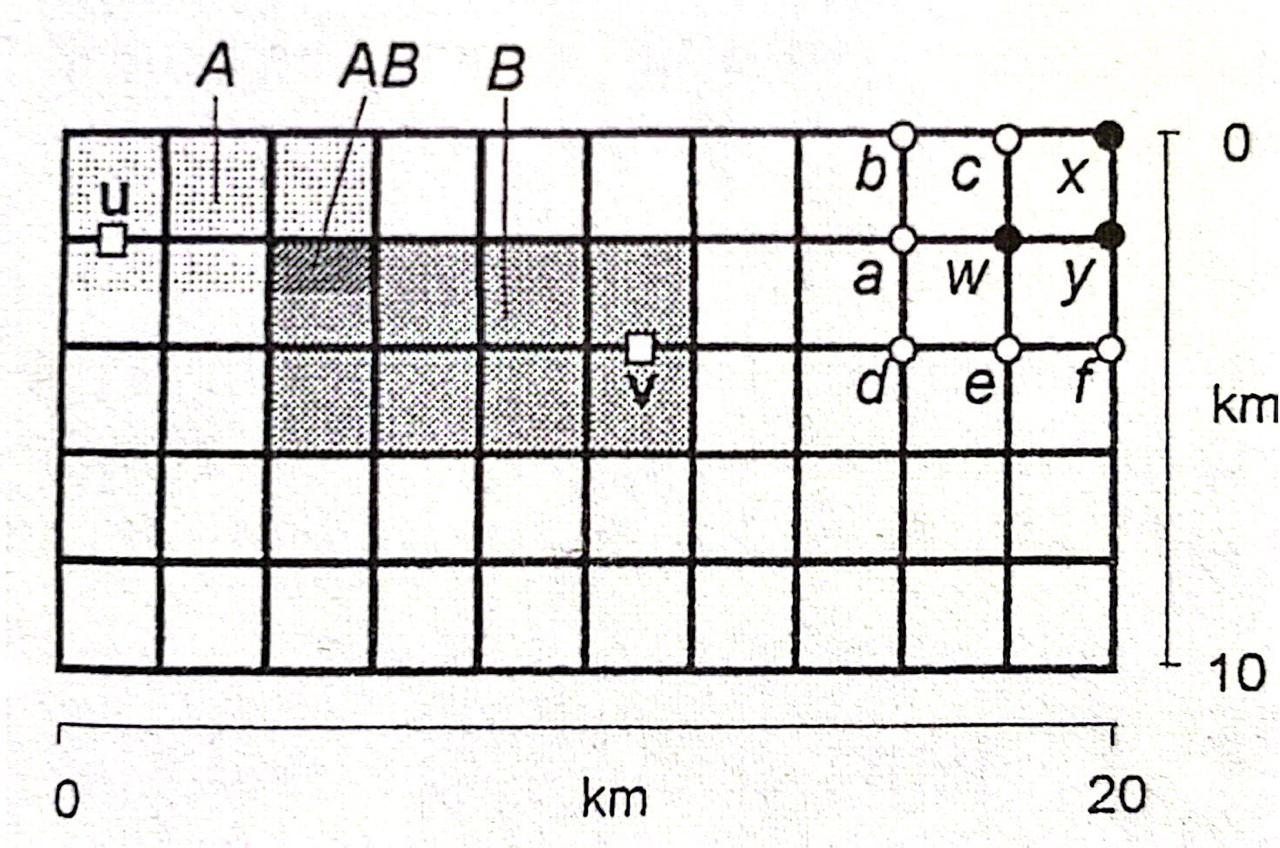
\includegraphics[width=0.9\textwidth]{fi223.jpeg}
        Suppose that an engineer is interested to analyse two events: $A \equiv \{ \text{a severe water loss occurs in location } \mathbf{u} \equiv (u_1 , u_2) \text{ where } 0 < u_1 \leq 6 \ km, 0 < u_2 \leq 3 \ km\}$, and   $B \equiv \{ \text{a severe water loss occurs in location } \mathbf{v} \equiv (v_1 , v_2) \text{ where } 4 < v_1 \leq 12 \ km, 2 < v_2 \leq 6 \ km\}$. The probability of occurrence of $A$ and $B$ is proportional to the area corresponding  (see the figure) to each event:
        $$
        Pr[A] = \frac{(6 x 3)}{200} = 0.09 \quad Pr[B] = \frac{(12 - 4) x (6 - 2)}{200} = \frac{8 x 4}{200} = 0.16
        $$
        Suppose that one want to know the probability of event $A$, given that a loss occurs in the area affected by $B$. To estimate this, it is needed to know the area affected by $B$ within which $A$ also occurs. The area for the event $AB$ is $(6 - 4) x (3 - 2) \ = \ 2 \ km^2 $. $Pr[AB]$ can be calculated as $Pr[AB] = \frac{2}{200} = 0.01$, or following the addition rule as:
$$
Pr[AB] = Pr[A] + Pr[B] - Pr[A + B] = 0.09 + 0.16 - \frac{48}{200} = 0.01
$$
Using the condition probability definition, the probability of $Pr[A | B]$ is:
    $$
    Pr[A | B] = \frac{Pr[AB]}{Pr[B]} = \frac{0.01}{0.16} = 0.0625
    $$
    \end{exampleblock}
\end{frame}

\subsection{Stochastic independence}
\begin{frame}{Stochastic independence}
    When the ocurrence of an event $A$ is not affected by the ocurrence of an event $B$, the two events are \emph{stochastically independent}. This means that:
    $$
    Pr[A | B] = Pr[A] \quad \text{ if } Pr[B] > 0 \text{ and } Pr[B | A] = Pr[B] \quad \text{ if } Pr[A] > 0
    $$
    According to conditional probability, if $A$ and $B$ are independent:
    $$
    Pr[A \cap B] = Pr[AB] = Pr[A] Pr[B]
    $$
    This equation means that the probability of the joint occurrence of two independent events $A$ and $B$ is equal to the product of their marginal probabilities. According to addition rule, for two idependent events $A$ and $B$, the probability of the union of the two (or more) events is:
    $$
    Pr[A + B] = Pr[A] + Pr[B] - Pr[A] Pr[B]
    $$
\end{frame}

\begin{frame}{Stochastic independence}
    \begin{exampleblock}{Dam reliability}
        Let's consider again the example given before, where a dam's failure can be caused because of either a flood exceeding the design capacity of the spillway (event $A$) or an earthquake that trigger the dam's collapse (event $B$). Recall that the probabilities of occurrence of $A$ and $B$ in a year are give by $Pr[A] = a$ and $Pr[A] = b$, respectively. If $A$ are $B$ independent events, their joint probability is $Pr[AB] = Pr[A] Pr[B] = ab$. The probability of the dam's failure is given by the probability of the union 
        \vspace{-5pt}
        $$
        Pr[A + B] = Pr[A] + Pr[B] - Pr[AB] = a + b - ab 
        \vspace{-5pt}
        $$
        For $a = 0.02$  and $b = 0.01$, $Pr[A + B] = 0.0298$. This value is very close to 0.03 resulted after using the Boole's inequality because the joint probability of the two events plays a minor role in risk assessment. 
        \begin{minipage}{0.7\textwidth}
            The sample space of this experiment is shown in the figure and it is constituted as $\Omega \equiv \{ AB, A B^c , A^c B , A^c B^c \}$. The dam's failure is represented by $A + B = (AB) \cup (A B^c ) \cup (A^c B )$. Conversely, the probability of dam's continuance is $Pr[A^c B^c ] = 1 - Pr[A + B] = 1 - (a + b - ab) = 1 - (0.02 + 0.01 - 0.01 x 0.02) = 0.9702$. The probability of dam's continuance is more than 97\% in a year. 
        \end{minipage}
        \hfill
        \begin{minipage}{0.3\textwidth}
            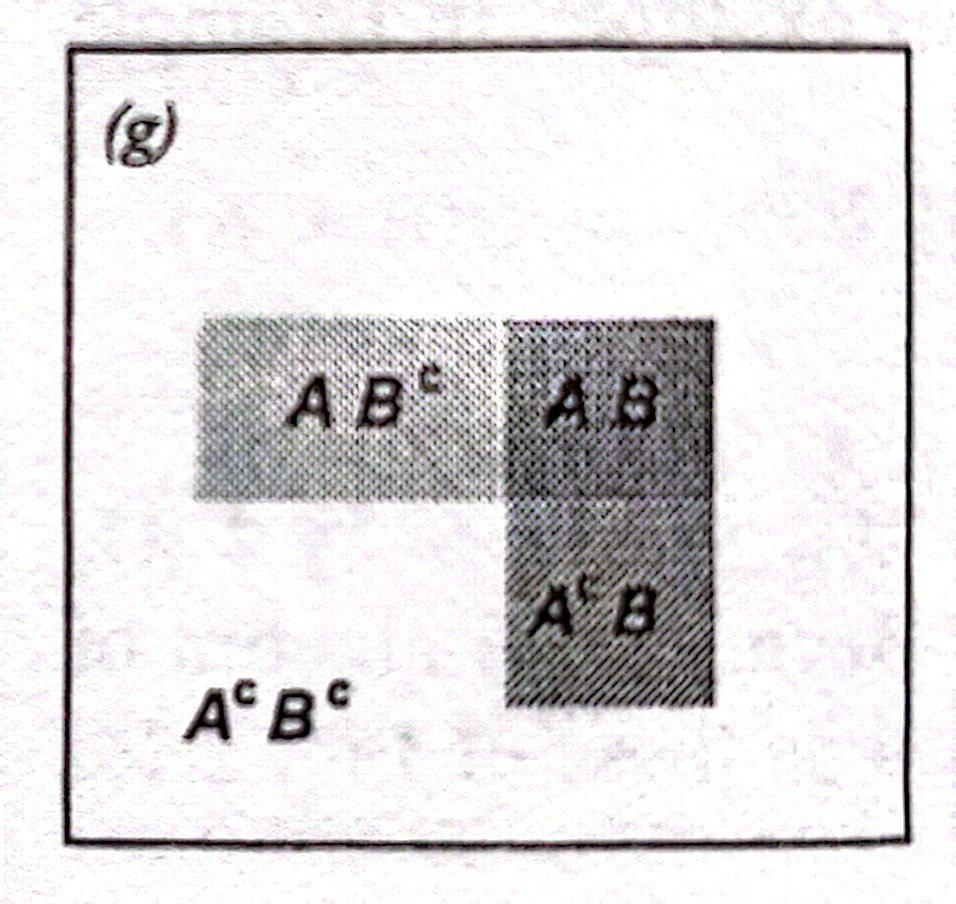
\includegraphics[width=\linewidth]{fi216g.jpeg}
        \end{minipage}
        Is the engineer is interested in knowing the dam's reliability during $m$ years (life time), the probability of failure must be estimated after $1, 2, \cdots, m$ years of the dam's construction. Accordingly, the dam's continuance after 1 year is $Pr[A^c B^c]$. As the experiment is repeated in subsequent years, la probability of survival after 2 years is: 
        \vspace{-5pt}
        $$
        Pr[(A^c B^c)_1 \cap (A^c B^c)_2] = Pr[(A^c B^c)_1 (A^c B^c)_2] = Pr[(A^c B^c)_1] Pr[(A^c B^c)_2 |  (A^c B^c)_1]
        \vspace{-5pt}
        $$
\end{exampleblock}
\end{frame}

\begin{frame}{Stochastic independence}
    \begin{exampleblock}{Dam reliability}
        Regarding that the events $A$ and $B$ occurring in given year are independent from those occurring in other year, following the definition of stochastic independence $Pr[(A^c B^c)_2 |  (A^c B^c)_1] = Pr[(A^c B^c)_2]$. This means that:
        \vspace{-5pt}
        $$
        Pr[(A^c B^c)_1 (A^c B^c)_2] = Pr[(A^c B^c)_1] Pr[(A^c B^c)_2]
        \vspace{-5pt}
        $$
        If the probability of dam's continuance is same year after year $Pr[(A^c B^c)_1 (A^c B^c)_2] = Pr[(A^c B^c)]^2 = [1 - (a + b - ab)]^2$. So that, the probability of dam's continuance after $m$ years is
        \vspace{-5pt}
$$
        Pr[(A^c B^c)_1 (A^c B^c)_2 \cdots (A^c B^c)_m] = Pr[(A^c B^c)]^m = [1 - (a + b - ab)]^m
        \vspace{-5pt}
        $$
        For $m = 50$, $Pr[(A^c B^c)_1 (A^c B^c)_2 \cdots (A^c B^c)_{50}] = 0.9702^{50} = 0.2203 $. This means that during the first 50 years the design has a realiability of 22\% whereas the risk of failure is 78\% (complementary probability). The risk of failure in the iht year is given by the probability that either $A$ or $B$ or both events ocurr in the ith year. This probability is given by:
        \vspace{-5pt}
        \begin{align*}
            Pr[(A^c B^c)_1 (A^c B^c)_2 (A^c B^c)_{i-1} \cdots (A + B)_i ] &= Pr[(A^c B^c)]^{i-1} Pr[(A + B)_i | (A^c B^c)_{i-1}] \\
                                                                          &= Pr[(A^c B^c)]^{i-1} Pr[(A + B)_i] \\
                                                                          &= [1 - (a + b - ab)]^{i-1} (a + b - ab)
        \end{align*}
        \vspace{-5pt}
     \end{exampleblock}
        \vspace{-15pt}
        \begin{minipage}{0.7\textwidth}
   As we have seem before, this probability represent the design realiability rescaled by the risk of failure. For instance, the probability of failure after 10 years of operation is:
    $$
    Pr[(A^c B^c)_1 (A^c B^c)_2 \cdots (A^c B^c)_{9} (AB)_{10} ] = 0.9702^9 x 0.0298 = 0.0227.  
    $$
        \end{minipage}
        \hfill
        \begin{minipage}{0.3\textwidth}
            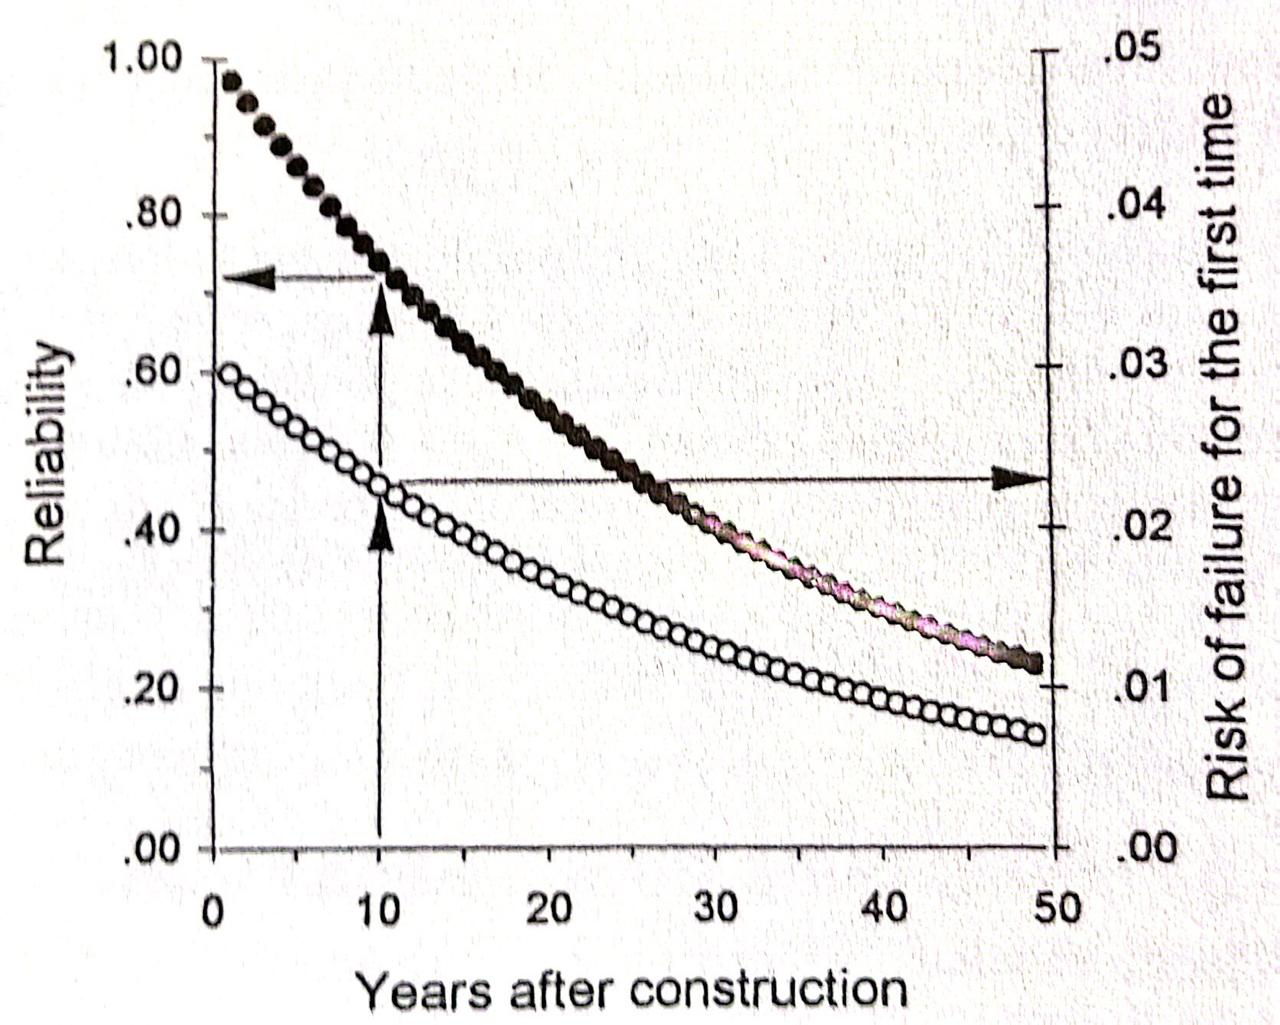
\includegraphics[width=\linewidth]{fi224.jpeg}
        \end{minipage}
\end{frame}

\subsection{Total probability and Bayes' theorems}
\begin{frame}{Total probability and Bayes' theorems}

    \begin{block}{Total probability}
        Sometimes the probability of an event $A$ can no be obtanined directly but, it can be estimated based on the probabilities of the occurrence of other events $B_i$ where $i = 1, 2, \cdots, n$. The probability of $A$ will thus depend on which of the $B_i$ events has ocurred and it will be the expected probability which is the average probability weighted by those of $B_i$. Consider $n$ $B_i$ mutually exclusive and collectively exhausted events where $i = 1, 2, \cdots, n$ and $B_i B_j = \varnothing$ for $i \neq j$, and $B_1 + B_2 + \cdots + B_n = \Omega$.

        \begin{minipage}{0.7\textwidth}
            The probability of other event $A$ (see the figure) can be given by:
        \begin{align*}
            Pr[A] &= Pr[A B_1 ] + Pr[A B_2 ] + \cdots + Pr[A B_n ] = \sum_{i=1}^n Pr[A B_i] \\
                  &= \sum_{i=1}^n Pr[A | B_i ] Pr[B_i] 
        \end{align*}
        \end{minipage}
        \hfill
        \begin{minipage}{0.3\textwidth}
            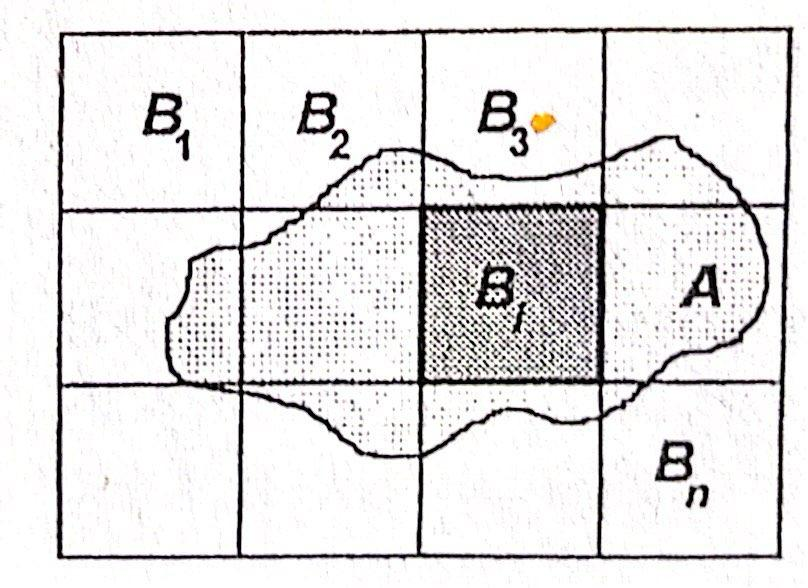
\includegraphics[width=\linewidth]{fi225.jpeg}
        \end{minipage}
        This expression is known as the \emph{theorem of total probability}. In words, this theorem indicates that the probability of an event $A$ that ocurr concurrently with a set of multiple $B_i$ events  is equal to the sum of the conditional probability of $A$ given $B_i$ and the marginal probability of $B_i$.
    \end{block}
\end{frame}

\begin{frame}{Total probability and Bayes' theorems}
    \begin{block}{Bayes' theorem}
        From the theorem of total probability, it might be of interest to estimate the probability of $B_j$ given the ocurrence of an event $A$. According to the conditional probability definition:
        $$
        Pr[B_j | A] = \frac{Pr[B_j A]}{Pr[A]}
        $$
        if the joing probability is $Pr[B_j A] = Pr[A | B_j] Pr[B_j]$, replacing in the equation above:
        $$
        Pr[B_j | A] = \frac{Pr[A | B_j] Pr[B_j]}{Pr[A]}
        $$
        According to the total probability theorem for $Pr[A]$ and replacing in the equation:
        $$
        Pr[B_j | A] = \frac{Pr[A | B_j] Pr[B_j]}{\sum_{i=1}^{n} Pr[A | B_i ] Pr[B_i]}
        $$
        This equation is known as the \emph{theorem of Bayes}. 
    \end{block}
\end{frame}

\begin{frame}{Total probability and Bayes' theorems}
    \begin{exampleblock}{Water quality}
        Consider the concurrent data of dissolved oxygen (DO) and biochemical oxygen demand (BOD) recorded in 38 sites on the Blackwater River, England (see table). It is assumed that the samples are taken from the same population given the similarities in water usages. According to the data means ($\mu$) of 7.5 mg/l and 3.2 mg/l, respectively, the following mutually exclusive and collectively exhaustive events are defined (see figure):
        \begin{minipage}{0.7\textwidth}
        \begin{align*}
            & B_1 \equiv \{ DO \leq 7.5 \text{ mg/l, } BOD > 3.2 \text{ mg/l} \} \\
            & B_2 \equiv \{ DO > 7.5 \text{ mg/l, } BOD > 3.2 \text{ mg/l} \} \\
            & B_3 \equiv \{ DO > 7.5 \text{ mg/l, } BOD \leq 3.2 \text{ mg/l} \} \\
            & B_4 \equiv \{ DO \leq 7.5 \text{ mg/l, } BOD \leq 3.2 \text{ mg/l} \}
        \end{align*}
        \end{minipage}
        \hfill
        \begin{minipage}{0.7\textwidth}
            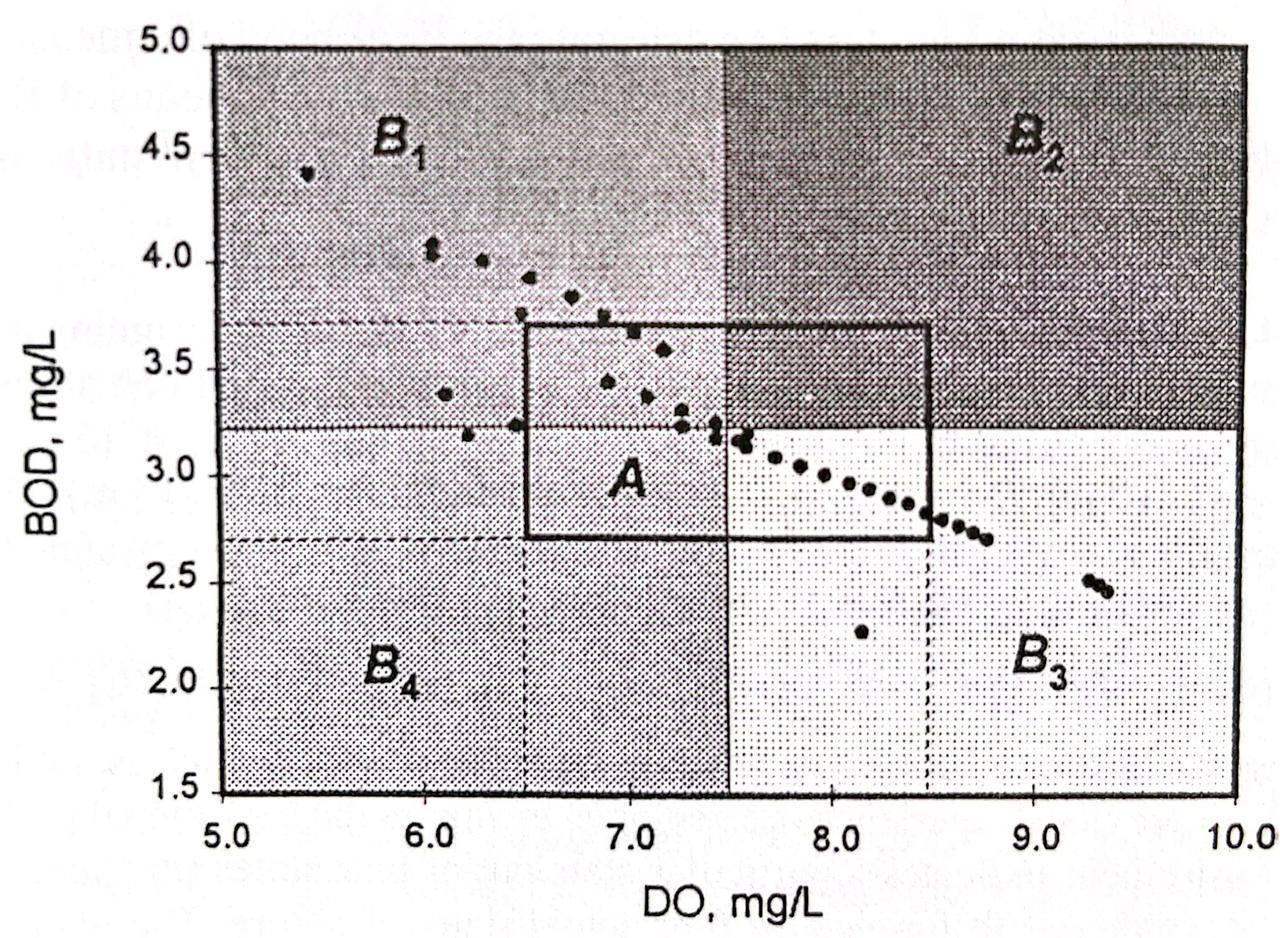
\includegraphics[width=\linewidth]{fi228.jpeg}
        \end{minipage}
        By using relative frequencies (see figure), $Pr[B_1] = 17/38 = 0.45$, $Pr[B_2] = 0/38 = 0$,$Pr[B_3] = 19/38 = 0.50$ and $Pr[B_4] = 2/38 = 0.05$. The standard deviations ($\sigma$) of DO and BOD data sets are 1.0 mg/l and 0.5 mg/l, respectively. Let $A$ be the event defined by the concurrent values of DO and BOD within the range $\mu \pm \sigma$ so:
        $$
        A \equiv \{ 6.5 < DO < 8.5 \text{ mg/l, } 2.7 < BOD < 3.7 \text{ mg/l} \}
        $$
Accordingly, the conditional probabilities of event $A$ given $B_i$ are $Pr[A | B_1] = 7/17 = 0.41$, $Pr[A | B_2] = \text{is undefined as } Pr[B_2] = 0$, $Pr[A | B_3] = 11/19 = 0.58$ and $Pr[A | B_4] = 1/2 = 0.5$. 
    \end{exampleblock}
\end{frame}

\begin{frame}{Total probability and Bayes' theorems}
    \begin{exampleblock}{Water quality}
        According to the total probability theorem, $Pr[A] = Pr[A | B_1] Pr[B_1] + Pr[A | B_2] Pr[B_2] +Pr[A | B_3] Pr[B_3] +Pr[A | B_4] Pr[B_4]$, replacing in this expression $Pr[A] = \frac{7}{17} x \frac{17}{38} + \text{ undefined } x 0 + \frac{11}{19} x \frac{19}{38} + \frac{1}{2} x \frac{2}{38} = \frac{7}{38} + \frac{11}{38} + \frac{1}{38} = \frac{19}{38} = 0.5 $. This means that the monitored vales of DO and BOD have a 50\% of chance of lying in range defined for the $A$ event. Using the Bayes's theorem:
        \vspace{-8pt}
        $$
        Pr[B_1 | A] = \frac{Pr[A | B_1] Pr[B_1]}{\sum_{i=1}^{4} Pr[A | B_i ] Pr[B_i]} = \frac{(7/17)(17/38)}{19/38} = \frac{7}{19} = 0.37
        $$
        which means that if the monitored DO and BOD values lie in the previously defined range, there is a 37\% change that neither DO nor BOD exceed their sample means. Applying the Bayes' theorem for the other $B$ events, $Pr[B_2 | A] = 0$, $Pr[B_3 | A] = 0.05$ and $Pr[B_4 | A] = 0.58$. 
    \end{exampleblock}
    The Bayes' theorem is quite useful for experiment performed in stages. The theorem is useful to update event probabilities in an experiment with continuos incorporation of data. By updating the prior probabilities, the engineer can assess the likelihood of design events by incorporating the additional information given by conditioned posterior probabilities. If one define as \emph{state} the unknown quantification of the \emph{population} and considers that some \emph{sample} of observations is available, Bayes' theorem can be written as:
    \vspace{-10pt}
    $$
    Pr[state | sample] = \frac{Pr[sample | state] Pr[state]}{\sum_{\text{all states}} Pr[sample | state] Pr[state] }
    $$
    In practice, the engineer has prior knowledge about the occurrences of different states of a population. Using the Bayes' theorem one can estimate the conditional probability of a given state of that population after a sample has been observed. 
\end{frame}

%-------
% From Kotte
\section{Random variables and probability distributions}
\begin{frame}{Random variables and probability mass function}
    \begin{block}{Random variables}
        A \emph{random variable} $X$ is any (physical) observed quantity whose posibilities of having a value $x$ are dictated according to a probability distribution. A random variable such as daily precipitation or instataneous streamflow are \emph{uncertain} or \emph{unpredictable} or \emph{nondeterministic}. Each outcome of a random variable or each simple event defined in a sample space, correspond to a numerical value of the random variable. A random variable $X$ can be viewed as a function that associate a real number with each and every elementary event in a sample space $\Omega$ of an experiment. $X$ is thus a real-value function defined on a sample space.  
    \end{block}
    
    \begin{block}{Probability mass function (pmf)}
        A random variable $X$ can be statistically described by its probability function which is a mathematical function. $X$ can be discrete or continuos random variable. A discrete random variable takes discrete values usually from the posive integer set (e.g. the number rainy days in a given month). The probability functio of a discrete random variable $X$ is known as the \emph{probabily mass function (pmf)} which is defined as $p_X (x) = Pr[X = x]$. The pmf of $X$ gives the point probabilities of the values taken $X$. The probability axioms mentioned before also apply here:
        \vspace{-6pt}
        \begin{align*}
            & 0 \leq p_X (x) \leq 1, \text{   for all possible x}\\
            & p_X (x) = 0, \text{   for all unrealizable x} \\
            & \sum p_X (x) = 1, \text{   which is assumed over all possible x}
        \end{align*}
        %\vspace{-6pt}
    So if one is certain that $X = x = c$, $Pr[X = c] = 1$. For $n$ mutually exclusive events $x_1$, $x_2$, $\cdots$, $x_n$, $p_X (x_1 + x_2 + \cdots + x_n) = p_X (x_1) + p_x(x_2) + \cdots + p_X (x_n)$.
    \end{block}
\end{frame}

\begin{frame}{pmf example}

    \begin{exampleblock}{Flood occurrence}
        Consider the number of floods per year for a period of 34 years in the Magra River at Calamazza, located between Pisa and Genoa. A flood occurs when mean daily streamflows overcome a threshold equal to 300 m$^3$/s (see the table). The pmf is shown in the figure.
        \begin{minipage}{0.49\textwidth}
            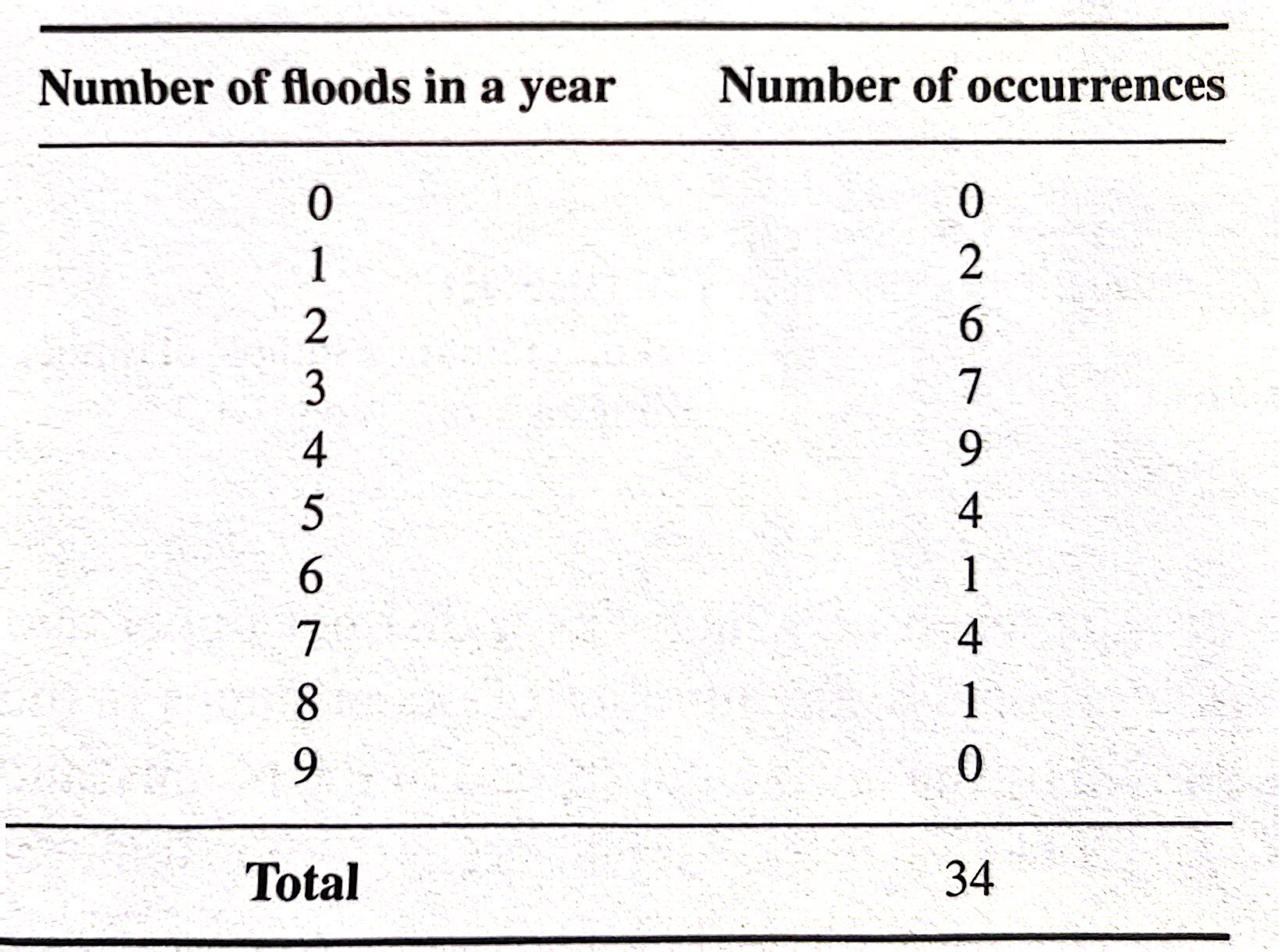
\includegraphics[width=\linewidth]{ta111.jpeg}
        \end{minipage}
        \hfill
        \begin{minipage}{0.5\textwidth}
            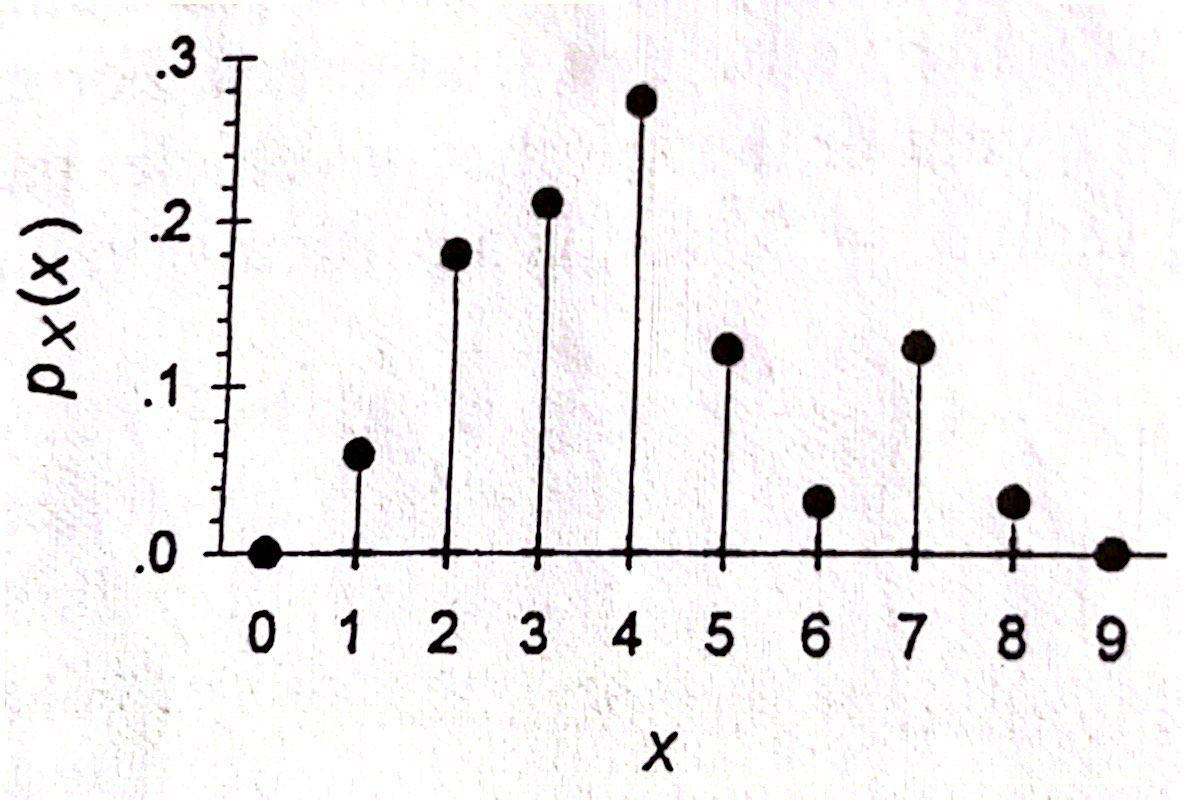
\includegraphics[width=\linewidth]{fi311.jpeg}
        \end{minipage}
    Note that in the figure,  $p_X(x) =\frac{\text{Number of occurrences}}{\text{Total of occurrences} = 34}$. 
    \end{exampleblock}    

\end{frame}

\begin{frame}{Cumulative distribution function (cdf) and cdf example} 
    \begin{block}{Cumulative distribution function}
        For a discrete or continuous random variable, the \emph{cumulative distribution function}, cdf, is the probability of nonexceedance of $x$ and is denoted by $F_X (x)$. The cdf is sometimes known as the \emph{distribution function}. $F_X (x) = Pr[X \leq x]$ so $F_X (x)$ is monotonic function that is bounded by 0 and 1, so $0 \leq F_X (x) \leq 1, \text{for all possible } x$. In the case of a discrete variable:
        \vspace{-9pt}
        $$
        F_X (x) = \sum_{ X_k \leq x } p_X(x_k)
        \vspace{-7pt}
        $$
        where $x_k$ represent all possible values of $X$ less than $x$. 
    \end{block}

    \begin{exampleblock}{Flood occurrence}
        Consider the example of the flood occurences per year given before. The pmf is shown in the figure.
            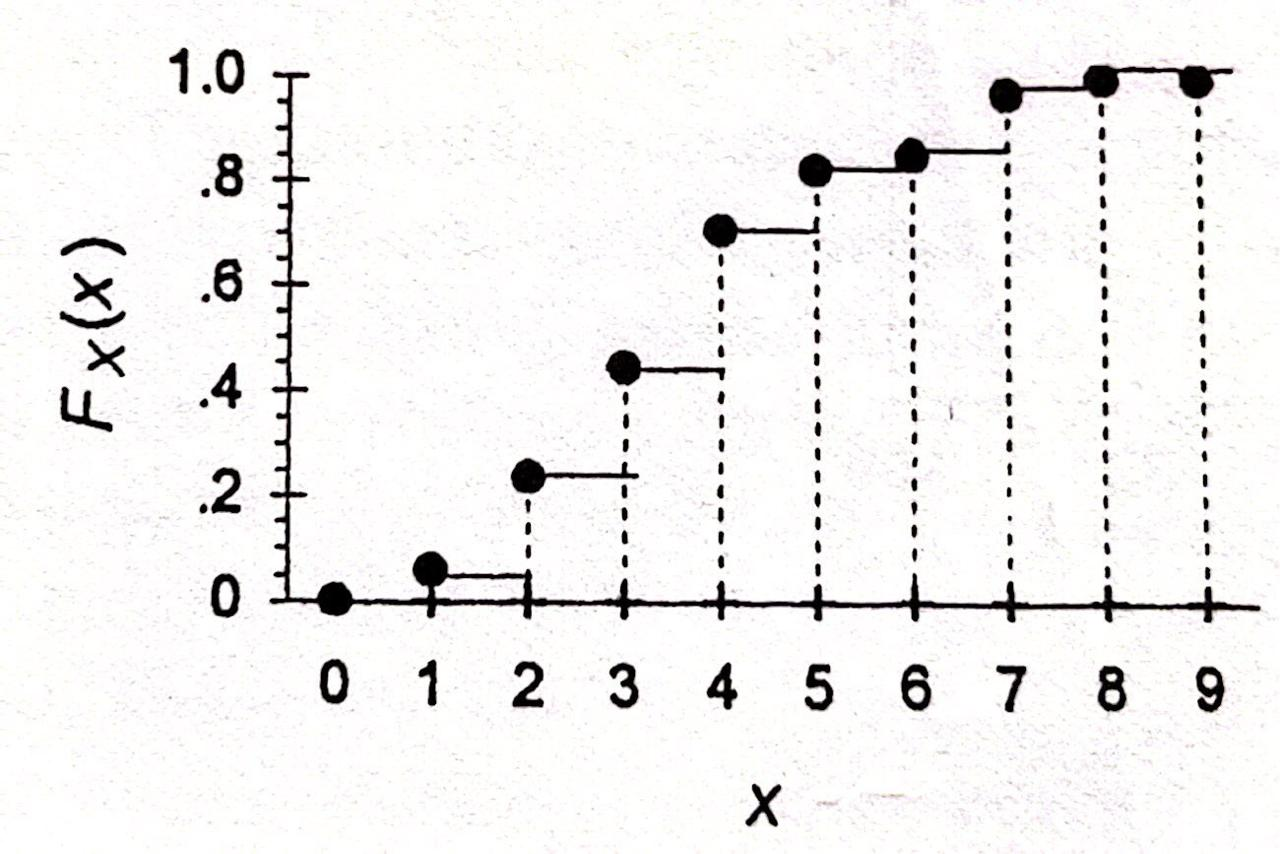
\includegraphics[width=\linewidth]{fi312.jpeg}
    \end{exampleblock}    
\end{frame}

\begin{frame}{Probability density function (pdf) and cumulative distribution function (cdf)} 
    
    \begin{block}{Probability density function (pdf)} 
        A random variable $X$  can take any value $x$ depending on the physical phonomena or quantity described and the accuracy of the measuring device (e.g. flow gauge). The probability llaw that describe the behaviour of a continuos random variable $X$ is given by the \emph{probability density function}, pdf. The pdf is denoted as $f_X (x)$ and is a nonnegative and continuos mathematical function over a range of values that $X$ can possibly take. $f_X (x)$ does not represent a probability because it is not dimensionless function. The probability that $X$ fall between $x_1$ and $x_2$ is given by:
        $$
        Pr[x_1 \leq X \leq x_2] = \int_{x_1}^{x_2} f_X (x) dx \leq 1.
        $$
        When $x_1$ and $x_2$ get closer, the probability above tend to zero which means that the probability that $X = c$ (take an specific value) is null. Some properties of a pdf are:
        \begin{align*}
            \int_{-\infty}^{\infty} f_X (x) dx &= 1 \\
            Pr[X > x] = \int_{x}^{\infty} f_X (x) dx &= 1- Pr[X \leq x]
        \end{align*}
    \end{block}
\end{frame}

\begin{frame}{Probability density function (pdf) and cumulative distribution function (cdf)} 
    \begin{block}{Cumulative distribution function (cdf)} 
        For a continuos random variable $X$, the cumulative distribution function, defined as the probability of nonexceedance within the range 0 to 1, is calculated as:
        \vspace{-9pt}
        $$
        F_X (x) = Pr[X \leq x] = \int_{-\infty}^{x} f_X (x) dx
        $$
        it follows that:
        $$
        \frac{d F_X (x)}{dx} = f_X (x)
        $$
    \end{block}
            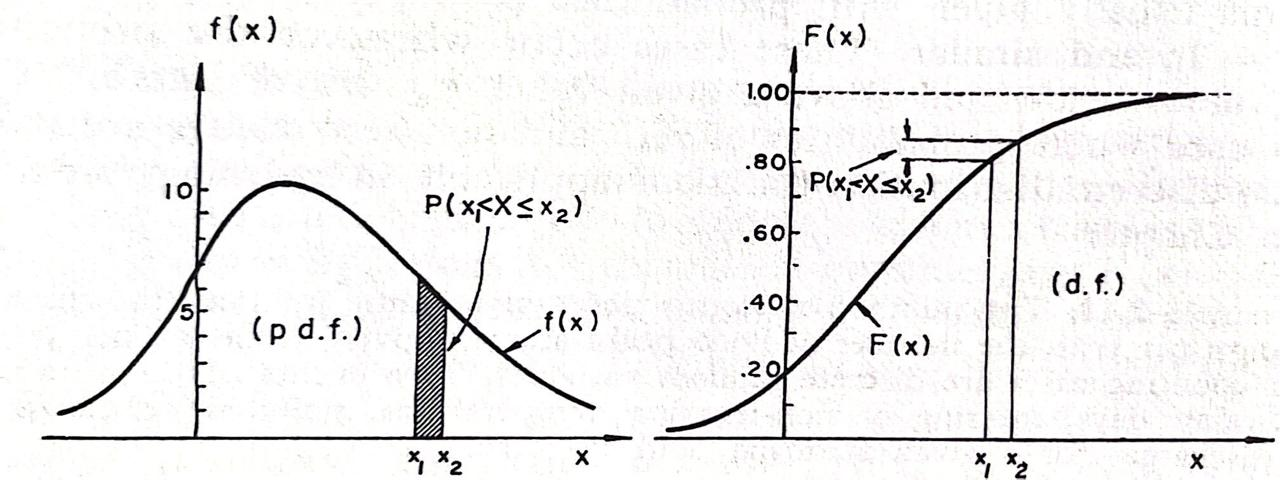
\includegraphics[width=\linewidth]{fiV23.jpeg} % From Vujika
\end{frame}

\begin{frame}{Probability density function (pdf) and cumulative distribution function (cdf)} 
    
    % Example 1.8 from Mario DG
    \begin{exampleblock}{Evaporation}
        Suppose that the pdf of the evaporation $V$ for any day of the year is defined as:
        \begin{minipage}{0.49\textwidth}
\[
f_V (v) = 
\left\{
\begin{array}{l}
    0.125 \text{, if } 0.5\leq v \leq 8.5 \ mm/day  \\
    0 = \text{ otherwise} 
\end{array}
\right.
\]
        \end{minipage}
        \hfill
        \begin{minipage}{0.39\textwidth}
            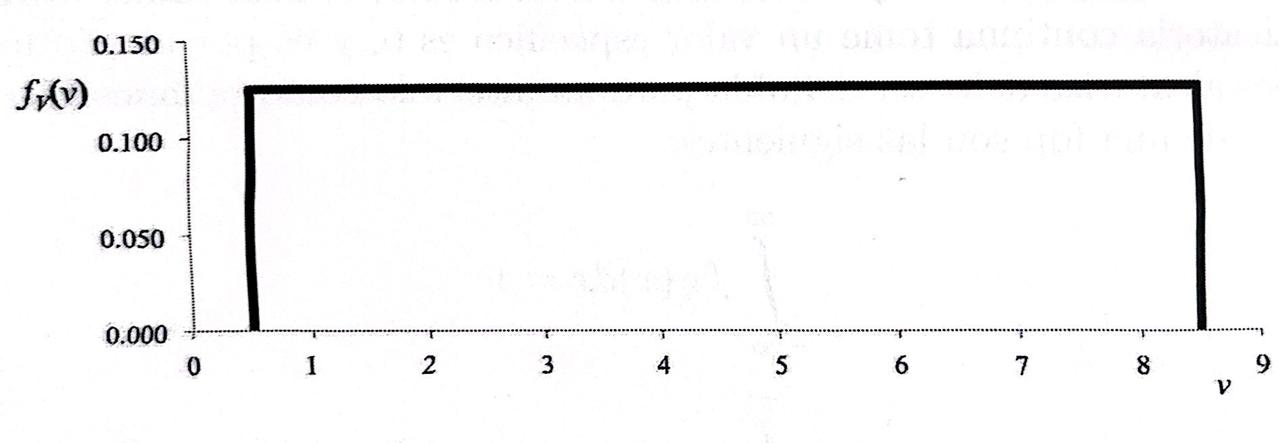
\includegraphics[width=\linewidth]{fiM18.jpeg}
        \end{minipage}
       To prove that this is a pdf, one can estimate the following:
       \[
           \int_{0.5}^{8.5} 0.125 dv = 0.125v \Big|_{0.5}^{8.5} = 0.125(8.5-0.5) = 1
       \]
       If one  want to know the probability that $4 \leq v \leq 6$ mm/day, one estimate:
       \[
           Pr[4 \leq v \leq 6] =  \int_{4}^{6} 0.125 dv = 0.125v \Big|_{4}^{6} = 0.125(6-4) = 0.25
       \]
       From the pdf, one can know the cdf as:
\[
    F_V (v) = Pr [V \leq v] = \int_{-\infty}^{v} f_V (v) = \int_{0.5}^{v} 0.125 dv = 0.125v - 0.0625 
       \]
       Accoring to this $Pr[V \leq 5.5] = 0.125(5.5) - 0.0625 = 0.625$ or the $Pr(V > 8,2] = 1 - (0.125(8.2) - 0.0625) = 0.0375$.
    \end{exampleblock}    
\end{frame}

\begin{frame}{Distribution of mixed variables} 
    \begin{block}{Distribution of mixed variables} 
        In hydrology is common to find random variables whose probability distribution is combined of both discrete (mass function) for one interval, and continuos (density function) for other interval. For instance, the distribution of an intermittent phenomena in hydrology, such as daily precipitation in an specific point where no precipitation fall for some days ($X = 0$), but when rain falls the value of $X > 0$ (see figure).

            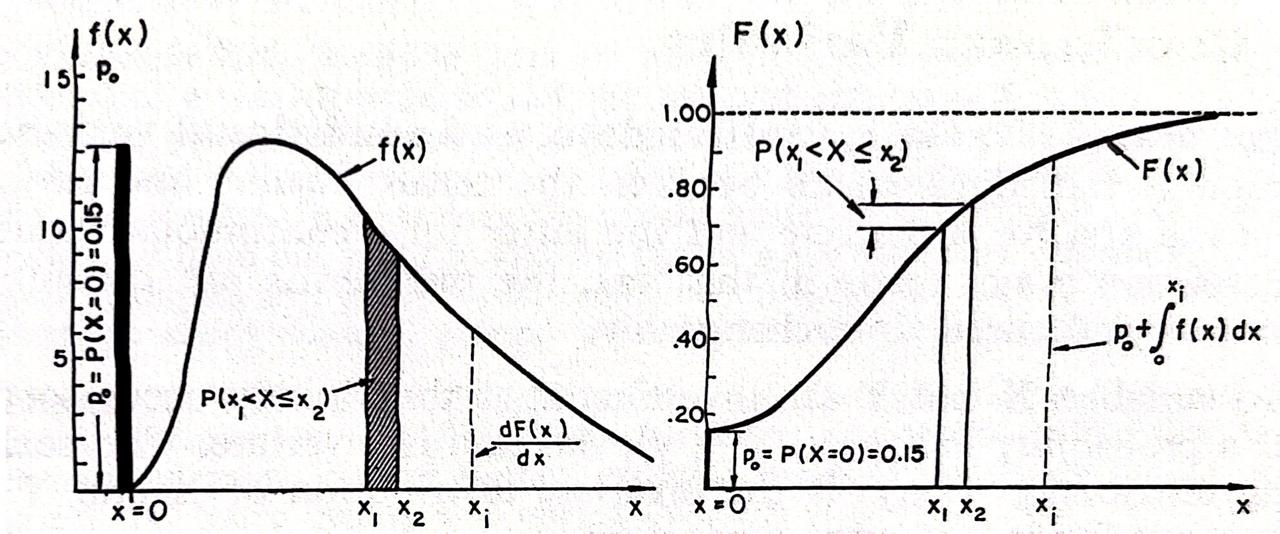
\includegraphics[width=0.8\linewidth]{fiV24.jpeg} % From Vujika

            This case is common whenever $X$ can be equal to zero or other boundaries besides all other continuous positive values. The probabilities can be estimated as 
            \[
            Pr[X\leq x] = Pr[X=0] + \int_{0}^{x} f_X (x) dx
            \vspace{-6pt}
        \]
            %\vspace{-6pt}
        However is not common practice to analyses hydrological random variables as mixed variables. Instead, sample spaces are designed to analyse discrete or continuous random variables. 
    \end{block}
\end{frame}
\end{document}
